% \begin{itemize}
%     \item \href{https://sci-hub.st/10.1007/s12243-021-00877-5}{A novel ofine indoor acoustic synchronization protocol: experimental analysis}: Another usage of de Bruijn sequence in synchronization.
%     \item \href{http://www-groups.mcs.st-andrews.ac.uk/~pjc/talks/21pmtia/pjc_pmtia2.pdf}{Synchronizing automata, de Bruijn graphs, and applications}:
%     \item \href{https://www4.comp.polyu.edu.hk/~comp2322/Bit\%20and\%20Frame\%20Synchronization\%20Techiques.pdf#:~:text=Synchronization\%20techniques\%20will\%20guide\%20the\%20receiving\%20system\%20in,the\%20need\%20for\%20error\%20control\%20at\%20higher\%20levels.}{Bit and Frame Synchronization
% Techniques}
% \end{itemize}
% {\color{red} A field where many application of de Bruijn sequences are found}
Transmitting, storing, protecting data (and so on) are challenging problems because of various factors: noisy channels, bandwidth, inter-symbol interference, $\ldots$. Coding theory is the study of the properties of codes and their fitness that helps dealing with these issues. In academic research, codes are involved in data-transmission, data-storage, data-compression, cryptography, error-detection and correction. 

\subsection{Brief overview}\label{subsec:brief_overview}
The article, "A Mathematical Theory of Communication" of Claude Shannnon, published in 1948, was considered to mark the birth of Coding Theory. In his work, Shannon showed that when a noisy communication channel is given, he defined a number, called the capacity of the channel, such that reliable communication can be achieved at any rate below the channel capacity, if proper encoding and decoding techniques are used. 


In more than half a century, coding theory has seen phenomenal growth. Many codes have been well-studied and have various application in real life. For example, Reed-Solomon code is used in 3G, 4G network, Turbo code is used in 5G network. Both Turbo code and LDPC code are channel coding technique that Data modems, telephone transmission, NASA Deep Space Network use to get the bit through. 

Usually, coding is divided into \textit{source coding} and \textit{channel coding}. 

Source coding plays a role of changing the message source to a code that is suitable for transmitting through the channel. For example, ASCII code is a source coding standard converting each character to a byte of 8 bits is an example of source coding. Another way to think about source coding is to treat it as a compress-decompress process. At the transmitter, the source encoder compresses the message for the purpose of economizing on the length of the transmission. At the other end, the source decoder decompresses the received signal or sequence. The commonly used compression algorithms include Huffman code used in JPEG, MPEG, MP3 files, Lempel-Ziv code used in ZIP files,$\cdots$.

Because of physical and engineering limitations, channels are not ideal: their output may differ from their input because of noise or manufacturing defects. The transmitted message may become distorted and the receiver might not realize that the message was corrupted. Additionally, there are applications, such as magnetic and optical mass storage media, where certain patterns are not allowed to appear in the channel's bit stream. The main role of channel coding is to overcome such limitations by encoding the message again after the source coding while maintaining the channel as transparent as possible from the source and destination points of view. 

\begin{figure}
    \centering
    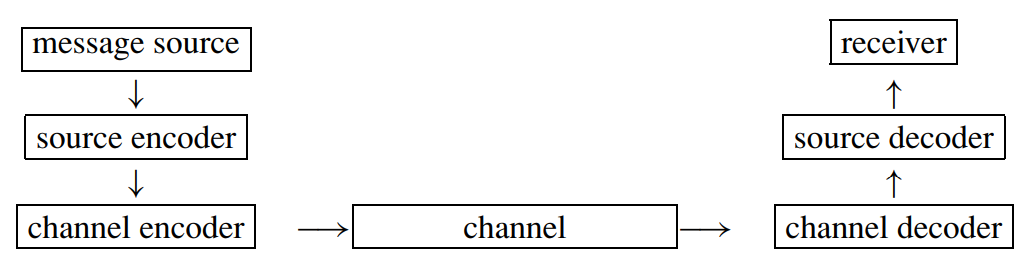
\includegraphics[scale=0.5]{fig/sourceandchannelcoding.png}
    \caption{Model of source and channel coding~\cite{ling2004coding}.}
    \label{fig:sourcechannelcoding}
\end{figure}

Section~\ref{subsec:brief_overview} has introduced to basic idea of coding theory. In the next section, this thesis provides the commonly used notations and terminologies of this research field.
\subsection{Notation and terminologies}
The most essential element of coding theory is \textbf{codeword}, which is a sequence of code symbols taken from a code alphabet
\begin{definition}[Code Alphabet]
    A code alphabet is set $\Sigma=\left\{a_{1},a_{2},\ldots,a_{q}\right\}$ of size $q$. The elements of $\Sigma$ are called code symbols, letters, and bits if $q=2$. A $q$-ary word of length $n$ over $\Sigma$ is a sequence (or string) $\bfw=w_{1}w_{2}\ldots w_{n}\in\Sigma^{n}$ with each $w_{i}\in\Sigma$ for all $i$. 
\end{definition}
In practice, the size of a code alphabet is often the size of a finite field, which is the power of a prime number. Hence, for simplicity, $\Sigma$ can be treated as a set of the first $q$ non negative integers without ambiguity. More particularly, the notation $\Sigma={0,1,2,\ldots,q-1}$ can be used instead.
\begin{definition}[Code and Codeword]
    A $q$-ary block code $C$ over $\Sigma$ is a nonempty set $C$ of $q-ary$ words of the same length $n$. Each element of $C$ is called a codeword in $C$.
\end{definition}
The study of a code $C$ involves the following process in an example of channel coding. Suppose that $\Sigma$ and $\Sigma^{\prime}$ are finite input and output of the channel respectively. Let $\bfm$, taken out of $M$ possible information words, be a message input to the channel encoder. Through a desired channel encoder, the message $\bfm$ is mapped to a longer codeword $\bfc\in\Sigma^{n}$. The word $\bfc$ is transmitted through the channel, become $\bfy\in\Sigma^{\prime n}$. After receiving $\bfy$, the role of the channel decoder is to produce codeword $\hat{\bfc}$ and a decoded information word $\hat{\bfu}$, aiming to have $\bfc=\hat{\bfc}$ and $\bfu=\hat{\bfu}$. Consequently, the mapping at the channel encoder needs to be one-to-one, and the size of the code $C$ is the maximal possible number of messages, or $\card{C}=M$.

Observe that, using code $C$, it takes a sequence of length $n$ to encode a sequence of length $\log_{\card{\Sigma}}(\card{C})$. In other words, $n-\log_{\card{\Sigma}}(\card{C})$ "redundant" bits were added to the message so that the channel can achieve its goal. Accordingly, a quantity concerning this redundancy was introduced, called \textit{(information) rate}. 
\begin{definition}[Information rate]\label{def:information_rate}
    The (information) rate of a code $C$ over an alphabet of size $q$ is defined as:
    \begin{align}
        R_{C}= \dfrac{\log_{q}(\card{C})}{n}.
    \end{align}
\end{definition}

Works in coding theory, including this thesis, are interested in designing codes with high rate, along with its efficient encoder, decoder, that can be used in specific situations. 

Based on their motive or their intrinsic properties, codes are categorized into linear codes, constrained codes, error-correcting codes, error-detecting codes,$\ldots$. This thesis focus on the combination of a constrained code, run length limited, and positioning code. A brief introduction to constrained code is given in the next section.

\subsection{Constrained code}\label{subsec:constrained_code}
Constrained Code is a sub-field of Coding theory, studies to design codes satisfying given constrained. The inspiration for the research of constrained codes comes from real problems. The transmitted data needs to follow some given standards which are necessary for the code to surmount the flaw of the environment. For instance, in the CD disc storage, errors tend to occur when there is a sequence of many consecutive $0$ bits. Consequently, it's crucial to construct codes that should avoid a long sequence of $0$ bits. A famous code invented to overcome this challenge is \gls{RLL} code by Immink~\cite{immink1990runlength}. \gls{RLL} codes are defined by $2$ parameters: $d, k$, and denoted by $(d,k)$-RLL, where $d$ and $k$ are two non-negative integers such that $d\leq k$. A finite length binary sequence 
is said to satisfy the $(d,k)$-RLL constraint if its number of $0$'s between $2$ consecutive $1$ bits is at least $d$ and at most $k$.

Illustration is a very convenient way to begin understanding things. In constrained code, a graph, usually called labeled graph, is a helpful visualization technique. More particularly, a labeled graph is a directed graph with its vertices and edges labeled. Vertices in labeled graph are also called states. And the start and end vertices of a directed edge are called initial and terminal states respectively. Given a state $v$, in-edges of $v$ are edges treating $v$ as terminate state. Similarly, out-edges of $v$ are edges taking $v$ as initial state. 

For example, the graph in figure~\ref{fig:d_k_RLL} represents a $(d,k)$-RLL code. It can be verified that a sequence $w$ satisfies the $(d,k)$-RLL constraint if and only if a path whose edge labeling is $w$ exists in the graph.

\begin{figure}[htbp]
    \centering
    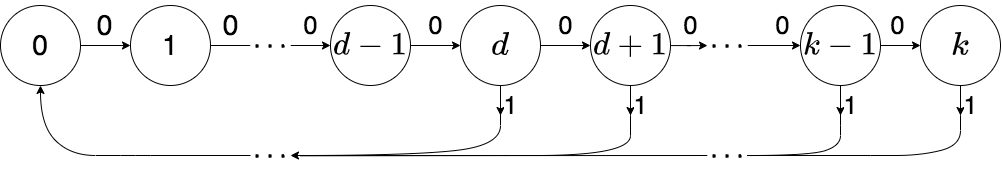
\includegraphics[scale=0.4]{fig/RLL.png}
    \caption{Graph representation of $(d,k)$-RLL code.}
    \label{fig:d_k_RLL}
\end{figure}

Labeled graphs are however more than just visualization tools. Using finite state splitting algorithm, they become encoders. In a constrained system, a very common problem is designing an encoding algorithm, which maps arbitrary user sequences into sequences obeying the constraints. Nevertheless, it's crucial to note that there are many kinds of encoders, depending on their objectives. For instance, there are encoders not taking any sequences as input, their goal are just to generate sequences satisfying given constraints. Such encoders are focused in this thesis. 

Beside constrained code, another combinatorial object drawing many attentions in coding theory is positioning code, also known by the name de Bruijn code. The formal definition of this code and its important results are presented in the next section.

% {\color{blue}
% \begin{itemize}
%     \item What is coding (def + sth from Ling San's book)
%     \item Application of coding
%     \item What are interested element in Coding (combinatorial object, encoder, decoder)
%     \item Constrained Code (Graph presentation (remember to mention in-edge, in-coming edge), Ronny)
%     \item Notation and Terminology
% \end{itemize}
% Something about error correcting, decoding ...
% }



